
\section{Case Study: RNA-seq data}\label{li}
\subsection{Introduction}
This section provides a detailed analysis of data from a study by
\citet{Li08} designed to address a range of practical issues in
RNA-seq experiments:
\begin{enumerate}
\item How many annotated genes are detected in a single cell type?

\item What is the number of tags that is necessary for the analysis of
  differentially regulated genes under different experimental
  conditions?

\item To what extent can different mRNA isoforms be detected?

\item How can one quantify alternative splicing by using a single or
  combination of existing technologies?
\end{enumerate}
\citet{Li08} attempt to address all of these issues on an
androgen-sensitive prostate cancer cell model. We are interested
primarily in the second question, and the challenge of identifying
differentially regulated genes under different experimental
conditions. We will demonstrate the use of the \edgeR~package for
analyzing RNA-seq data for differential gene expression.

\subsection{Source of the data}
\citet{Li08} sequenced $\textrm{poly(A)}^+$ RNA from mock-treated or
androgen sensitive LNCaP cells (a cell line of human cells commonly
used in the field of oncology) on the Illumina 1G Genome Analyzer. The
researchers used a double-random priming approach that was capable of
generating strand-specific information, although this is not of
relevance to our analysis here. The raw RNA-seq data provided by Li et
al. consists of 7 `lanes' of 35bp reads.~\footnote{The Illumina
  instrument requires samples to be placed in a `flow cell' which
  contains eight `lanes'---each lane has a sample of cDNA and
  generates a library of sequence counts for that sample.}
Approximately 10 million sequence tags were generated from both
control and hormone-treated cells (treated with DHT), and
\citet{Li08}'s analysis suggests that this tag density is sufficient
for quantitative analysis of gene expression.

The 10 million sequenced tags arise from four libraries from control
cells and three libraries for hormone-treated cells, giving a total of
seven libraries to analyse. From \citet{Li08} and its companion paper
\citep{Li:2006p382} it is unclear as to whether the treatments are
independent or not. The following analysis shows how a quantitative
analysis of gene expression, focusing on identifying differentially
expressed genes, can be conducted for these seven libraries using
\edgeR.

\subsection{Reading in the data and creating a \code{DGEList} object}
Our first task is to load the \edgeR~package and read the data into
\R. In this case, the tag counts for the libraries are stored in a
single table in a plain text file \code{pnas\_expression.txt}, in
which the rows of the table represent tags and the columns represent
the different libraries.

To turn the raw RNA-seq data into a table of counts, reads were mapped
to the NCBI36 build of the human genome using \code{bowtie}, allowing
up to two mismatches. Reads which did not map uniquely were
discarded. The number of mapped reads that overlapped ENSEMBL gene
annotations (version 53) was then counted. In counting reads
associated with genes, reads which mapped to non-coding gene regions,
such as introns, were included in the count.

Unlike in the other datasets we have look at, counts here are
aggregated at the gene, not at the tag, level.

The \code{files} object provides the name of the data file, and makes
a convenient argument to the function \code{read.delim} which reads
the table of counts into our \R~session.

\begin{Schunk}
\begin{Sinput}
> path <- getwd()
> setwd("/Users/dmccarthy/Documents/DGE/LiData")
> library(edgeR)
> raw.data <- read.delim("pnas_expression.txt")
> names(raw.data)
\end{Sinput}
\begin{Soutput}
[1] "ensembl_ID" "lane1"      "lane2"      "lane3"      "lane4"     
[6] "lane5"      "lane6"      "lane8"      "len"       
\end{Soutput}
\begin{Sinput}
> setwd(path)
\end{Sinput}
\end{Schunk}

The raw data is stored in a table with columns representing the gene
names, the counts for the seven libraries and a column giving the
length of each gene. The gene length is not currently used by \edgeR,
but this information could be used in future versions of the
package. In the code below, we assign the counts matrix to an object
\code{d} with the appropriate rownames, define the groups to which the
samples belong, and then pass these arguments to \code{DGEList}, which
calculates the library sizes and constructs a \code{DGEList}
containing all of the data we require for the analysis. We filter out
lowly expressed tags and those which are only expressed in a small
number of samples. We keep only those tags that have at least one
count per million in at least three samples.

\begin{Schunk}
\begin{Sinput}
> d <- raw.data[, 2:8]
> rownames(d) <- raw.data[, 1]
> group <- c(rep("Control", 4), rep("DHT", 3))
> d <- DGEList(counts = d, group = group)
> dim(d)
\end{Sinput}
\begin{Soutput}
[1] 37435     7
\end{Soutput}
\begin{Sinput}
> d <- d[rowSums(1e+06 * d$counts/expandAsMatrix(d$samples$lib.size, 
+     dim(d)) > 1) >= 3, ]
> d <- calcNormFactors(d)
> d
\end{Sinput}
\begin{Soutput}
An object of class "DGEList"
$samples
        group lib.size norm.factors
lane1 Control   978576    1.0296636
lane2 Control  1156844    1.0372521
lane3 Control  1442169    1.0362662
lane4 Control  1485604    1.0378383
lane5     DHT  1823460    0.9537095
lane6     DHT  1834335    0.9525624
lane8     DHT   681743    0.9583181

$counts
                lane1 lane2 lane3 lane4 lane5 lane6 lane8
ENSG00000124208   478   619   628   744   483   716   240
ENSG00000182463    27    20    27    26    48    55    24
ENSG00000124201   180   218   293   275   373   301    88
ENSG00000124207    76    80    85    97    80    81    37
ENSG00000125835   132   200   200   228   280   204    52
16489 more rows ...

$all.zeros
ENSG00000124208 ENSG00000182463 ENSG00000124201 ENSG00000124207 ENSG00000125835 
          FALSE           FALSE           FALSE           FALSE           FALSE 
16489 more elements ...
\end{Soutput}
\end{Schunk}

This \code{DGEList} is now ready to be passed to the functions that do
the calculations to determine differential expression levels for the
genes.

\subsection{Producing an MDS plot}
Before proceeding with the computations for differential expression,
it is possible to produce a plot showing the sample relations based on
multidimensional scaling, as demonstrated for the Tag-seq data
above. We can produce an MDS plot for the Li Data using the command below.

\begin{Schunk}
\begin{Sinput}
> pdf(file = "edgeR_case_study_Li_MDSplot.pdf", height = 6, width = 6)
> plotMDS.dge(d, main = "MDS Plot for Li Data", xlim = c(-1, 1), 
+     labels = c("Control1", "Control2", "Control3", "Control4", 
+         "DHT1", "DHT2", "DHT3"))
\end{Sinput}
\begin{Soutput}
Using grid search to estimate tagwise dispersion. 
\end{Soutput}
\begin{Sinput}
> dev.off()
\end{Sinput}
\begin{Soutput}
null device 
          1 
\end{Soutput}
\end{Schunk}


The resulting plot for the Li data is shown in~\ref{fig:Li_MDS}. In
this plot, Dimension 1 clearly separates the Control from the
DHT-treated samples. This shows that the replicates are reasonably
similar to each other and that we can expect to find lots of DE
genes. Having now investigated some of the relationships between the
samples we can proceed to the DE analysis of the data.

\begin{figure}[ht]
\begin{center}
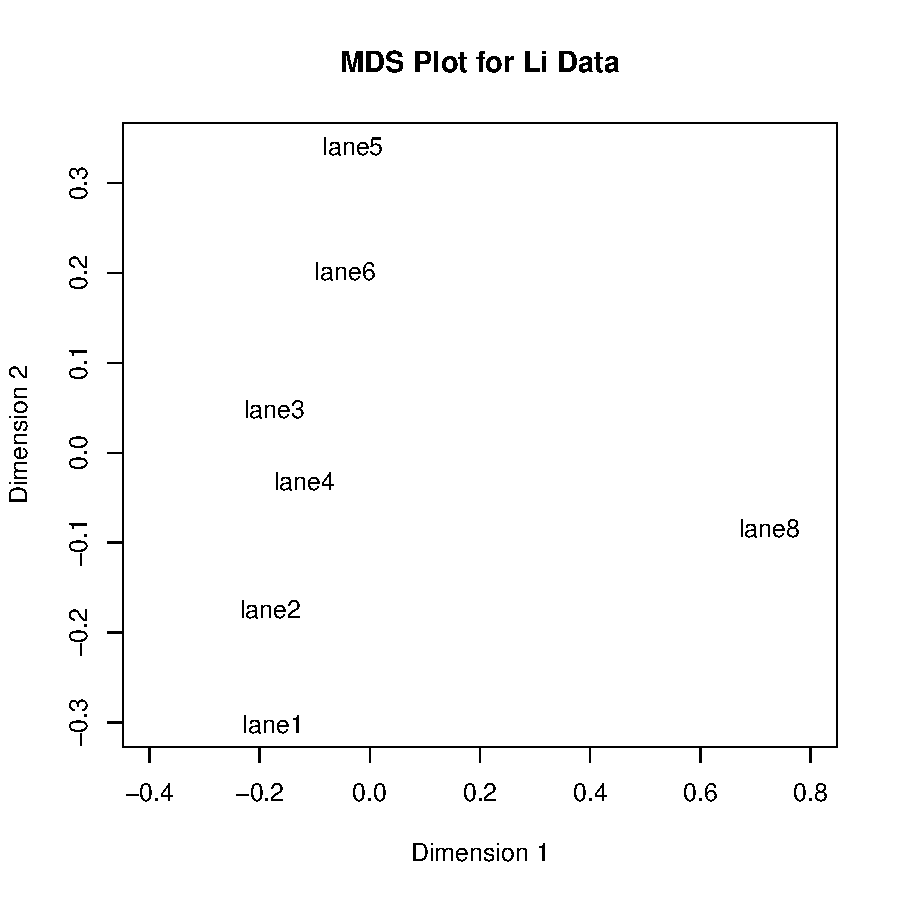
\includegraphics[height=0.45\textheight]{edgeR_case_study_Li_MDSplot.pdf}
\caption{Multidimensional scaling (MDS) plot for the Li data, showing
  the degree of similarity between the samples in two dimensions. We
  see that Dimension 1 strongly separates the Control from the
  DHT-treated samples. There are no outliers on this plot.}
\label{fig:Li_MDS}
\end{center}
\end{figure}


\subsection{Analysis using common dispersion}
\subsubsection{Estimating the common dispersion}
As discussed for the SAGE data, the first major step in the analysis
of DGE data using the NB model is to estimate the dispersion parameter
for each tag. Like in the earlier case study, we begin by estimating
the common dispersion using the function \code{estimateCommonDisp},
and analysing the data using the common dispersion.

\begin{Schunk}
\begin{Sinput}
> d <- estimateCommonDisp(d)
> names(d)
\end{Sinput}
\begin{Soutput}
[1] "samples"           "common.dispersion" "counts"           
[4] "pseudo.alt"        "genes"             "all.zeros"        
[7] "conc"              "common.lib.size"  
\end{Soutput}
\end{Schunk}

The output of \code{estimateCommonDisp} is a DGEList object with
several new elements. The element \code{common.dispersion}, as the
name suggests, provides the estimate of the common dispersion. The
pseudocounts calculated under the alternative hypothesis are given by
\code{pseudo.alt}. The element \code{conc} gives the estimates of the
overall concentration of each tag across all of the original samples
(\code{conc\$conc.common}) and the estimate of the concentration of
each tag within each group (\code{conc\$conc.group}). The element
\code{common.lib.size} gives the library size to which the original
libraries have been adjusted in the pseudocounts.

We see in the output below that the total counts in each library of
the pseudocounts agrees well with the common library size, as desired.

\begin{Schunk}
\begin{Sinput}
> d$samples$lib.size
\end{Sinput}
\begin{Soutput}
[1]  978576 1156844 1442169 1485604 1823460 1834335  681743
\end{Soutput}
\begin{Sinput}
> d$common.lib.size
\end{Sinput}
\begin{Soutput}
[1] 1276768
\end{Soutput}
\begin{Sinput}
> colSums(d$pseudo.alt)
\end{Sinput}
\begin{Soutput}
  lane1   lane2   lane3   lane4   lane5   lane6   lane8 
1237867 1228722 1229837 1227950 1336999 1338589 1332297 
\end{Soutput}
\end{Schunk}

Here the coefficient of variation of biological variation (square root
of the common dispersion) is found to be $0.142$. We also note that
although a common dispersion estimate of $0.02$ may seem `small', if a
tag has just an average of just $200$ counts per sample, then the
estimate of the tag's variance is 5 times greater than it would be
under the Poisson model.

\begin{Schunk}
\begin{Sinput}
> d$common.dispersion
\end{Sinput}
\begin{Soutput}
[1] 0.0199892
\end{Soutput}
\begin{Sinput}
> sqrt(d$common.dispersion)
\end{Sinput}
\begin{Soutput}
[1] 0.1413832
\end{Soutput}
\end{Schunk}

\subsubsection{Testing}
Once we have an estimate of the common dispersion, we can proceed with
testing procedures for determining differential expression. As for the
SAGE data, there are only two groups here, so the pair need not be
specified in the call to \code{exactTest}.

\begin{Schunk}
\begin{Sinput}
> de.com <- exactTest(d)
\end{Sinput}
\begin{Soutput}
Comparison of groups:  DHT - Control 
\end{Soutput}
\begin{Sinput}
> names(de.com)
\end{Sinput}
\begin{Soutput}
[1] "table"      "comparison" "genes"     
\end{Soutput}
\end{Schunk}

The results of the NB exact test can be accessed conveniently using
the \code{topTags} function applied to the object produced by
\code{exactTest}. The table below shows the top $10$ DE genes ranked
by $p$-value.

The table in the output from \code{topTags} shows that the
\edgeR~package identifies a great deal of differential expression, and
gives the top genes extremely small $p$-values, even after adjusting
for multiple testing. Furthermore, all of the top genes have a very
large fold change (indicating that these tags are likely to be
biologically meaningful), and all are up-regulated in the
DHT-treatment group compared to the control group.

Of course, for many applications the ranking for differential
expression is more important than the $p$-value, and \code{topTags}
provides such a ranking. As suggested in the SAGE case study, a Gene
Ontology analysis could be carried out using the list of top gene and
$p$-values provided by \code{topTags} in order to obtain more
systematic and functional information about the differentially
expressed genes.

\begin{Schunk}
\begin{Sinput}
> topTags(de.com)
\end{Sinput}
\begin{Soutput}
Comparison of groups: DHT-Control 
                  logConc    logFC        PValue           FDR
ENSG00000151503 -11.93976 5.822268 6.514565e-193 1.074512e-188
ENSG00000096060 -11.32470 5.010054 1.234621e-162 1.018192e-158
ENSG00000127954 -15.62463 8.236128 2.431779e-153 1.336992e-149
ENSG00000166451 -12.27934 4.687187 1.046604e-134 4.315670e-131
ENSG00000131016 -14.42053 5.307517 4.117750e-110 1.358363e-106
ENSG00000113594 -12.82529 4.117312 5.314184e-102  1.460869e-98
ENSG00000116285 -13.55908 4.205334  4.633316e-93  1.091742e-89
ENSG00000123983 -12.08741 3.661336  1.192773e-92  2.459200e-89
ENSG00000166086 -15.23730 5.508111  1.912744e-90  3.505422e-87
ENSG00000162772 -10.80873 3.318935  7.148502e-86  1.179074e-82
\end{Soutput}
\end{Schunk}

The table below shows the raw counts for the genes that \edgeR~has
identified as the most differentially expressed. For these genes there
seems to be very large differences between the groups, suggesting that
the DE genes identified are truly differentially expressed.

\begin{Schunk}
\begin{Sinput}
> detags.com <- rownames(topTags(de.com)$table)
> d$counts[detags.com, ]
\end{Sinput}
\begin{Soutput}
                lane1 lane2 lane3 lane4 lane5 lane6 lane8
ENSG00000151503    35    35    49    59  3307  3439  1224
ENSG00000096060    65    79   105   113  3975  3727  1451
ENSG00000127954     0     0     3     3   607   602   220
ENSG00000166451    41    52    57    57  1750  1654   728
ENSG00000131016     9     5    18     6   564   377   213
ENSG00000113594    37    36    57    43   936   959   418
ENSG00000116285    18    28    23    32   645   630   218
ENSG00000123983    62    76    94   108  1354  1258   628
ENSG00000166086     9     2     3     6   296   298   121
ENSG00000162772   172   204   250   304  2972  3269  1112
\end{Soutput}
\end{Schunk}

If we order the genes by fold change instead of $p$-value, we see that
the genes with the largest fold changes have very small
concentrations. This ranking is dominated by genes that have zero
total counts in one group and is less informative than ranking by
$p$-value.

\begin{Schunk}
\begin{Sinput}
> topTags(de.com, n = 10, sort.by = "logFC")
\end{Sinput}
\begin{Soutput}
Comparison of groups: DHT-Control 
                  logConc     logFC       PValue          FDR
ENSG00000091972 -31.78321 -36.46569 1.239501e-54 5.525493e-52
ENSG00000164120 -32.24356  35.54500 3.118964e-45 1.049881e-42
ENSG00000100373 -32.95621 -34.11968 1.066402e-16 5.729392e-15
ENSG00000118513 -33.03119 -33.96974 3.349294e-15 1.551777e-13
ENSG00000081237 -33.18303 -33.66604 1.411324e-12 4.646384e-11
ENSG00000196660 -33.24828 -33.53555 1.698009e-11 4.870776e-10
ENSG00000117245 -33.26382 -33.50448 2.846526e-11 7.928600e-10
ENSG00000019549 -33.36137  33.30938 2.364783e-13 8.388116e-12
ENSG00000059804 -33.40584  33.22043 1.021413e-12 3.403471e-11
ENSG00000018625 -33.41264  33.20683 2.131755e-12 6.814179e-11
\end{Soutput}
\end{Schunk}

We can see how many genes are identified as differentially expressed
between the control group (untreated LNCaP cells) and the DHT-treated
LNCaP cells, for a given threshold for the exact $p$-value or for the
adjusted $p$-value.

As the output below shows, \edgeR~detects a huge number of
differentially expressed genes in this dataset. Over $3000$ genes
are given a $p$-value less than $0.01$.

\begin{Schunk}
\begin{Sinput}
> summary(decideTestsDGE(de.com, p.value = 0.01))
\end{Sinput}
\begin{Soutput}
   [,1] 
-1  1620
0  13110
1   1764
\end{Soutput}
\end{Schunk}

The output below shows that $4936$ genes are given an adjusted
$p$-value of less than $0.05$. This means that if we set our control
the FDR for differential expression at 5\%, then \edgeR~identifies
$30$\% of all the genes in the dataset as differentially expressed.

\begin{Schunk}
\begin{Sinput}
> summary(decideTestsDGE(de.com, p.value = 0.05))
\end{Sinput}
\begin{Soutput}
   [,1] 
-1  2463
0  11558
1   2473
\end{Soutput}
\end{Schunk}

Of the genes identified as DE above, $2463$ ($49.9$\% of the DE genes) are
up-regulated in DHT-treated compared with control cells, and $2473$
($50.1$\%) are up-regulated in the control cells compared with DHT-treated
cells. It is interesting to note that although we detect far more
genes as DE that are up-regulated in the control group, all of the top
ten genes were up-regulated in the DHT-treated group.


\subsubsection{Visualising DGE results}
The code for producing the default fold-change plot, with the top
$500$ most DE tags highlighted in red, is shown below, and the result
of this code is shown in Figure~\ref{fig:Li_FC1}. In
Figure~\ref{fig:Li_FC1}, we see that the $500$ tags identified as most
differentially expressed have large fold changes---almost all of the
$500$ tags in red fall outside the blue lines at $\log \textrm{FC} =
-2$ and $\log \textrm{FC} = 2$. This means that most of these tags
show at least a 4-fold change in expression level between the
samples. This plot suggests strongly that the tags identified by
\edgeR~as differentially expressed are truly differentially expressed,
and, given the large changes in expression level, are likely to be
biologically meaningful.

\begin{Schunk}
\begin{Sinput}
> detags500.com <- rownames(topTags(de.com, n = 500)$table)
> png(file = "edgeR_case_study_Li-017.png", height = 600, width = 600)
> plotSmear(de.com, de.tags = detags500.com, main = "FC plot using common dispersion")
> abline(h = c(-2, 2), col = "dodgerblue", lwd = 2)
> dev.off()
\end{Sinput}
\begin{Soutput}
null device 
          1 
\end{Soutput}
\end{Schunk}

\begin{figure}[ht]
\begin{center}
\includegraphics[height=0.45\textheight]{edgeR_case_study_Li-017.png}
\caption{Plot of the log-fold change against the log-concentration for each tag. The $500$ most differentially expressed tags as identified by \edgeR~using the common dispersion are outlined in red.}
\label{fig:Li_FC1}
\end{center}
\end{figure}


\subsection{Analysis using moderated tagwise dispersions}
\subsubsection{Moderating the tagwise dispersion}
As discussed in the previous case studies, an extension to simply
using the common dispersion for each tag is to estimate the dispersion
separately for each tag, while `squeezing' these estimates towards the
common dispersion estimate. The goal of this moderation of the
dispersion estimates is to improve inference by sharing information
between tags. This type of analysis can be carried out in few steps
using the \edgeR~package.

To run the moderated analysis, we need to determine how much
moderation is necessary. As discussed above, we currently prefer to
choose a sensible value for the smoothing parameter \emph{a priori},
although we do have an algorithm developed by \citet{Robinson07} for
estimating the smoothing parameter as an approximate eBayes rule.

As we only have seven libraries, a small sample size, we should not be
too confident about the accuracy of the tagwise dispersions. Therefore
it is recommended to use a larger value for \code{prior.n}, which
can be selected \emph{a priori}, instead of being estimated. In an
experiment such as this, the seven samples mean that we have five
degrees of freedom for estimating the dispersion parameter. Thus,
setting the \code{prior.n} to be ten (as we have done previously)
should be appropriate. This means that the common likelihood receives
the weight of ten individual tags. Therefore, there will be a
reasonable degree of `squeezing' towards the common dispersion
estimate, but still enough scope to allow flexibility when estimatig
the individual dispersion for each gene.

The function \code{estimateTagwiseDisp} produces a DGEList object that
contains all of the elements present in the object produced by
\code{estimateCommonDisp}, as well as the value for \code{prior.n}
used (\code{d\$prior.n}) and the tagwise dispersion estimates
(\code{d\$tagwise.dispersion}), as we see below. Here we set
\code{grid.length=500} for greater precision in the tagwise dispersion
estimates.

\begin{Schunk}
\begin{Sinput}
> system.time(d <- estimateTagwiseDisp(d, prior.n = 10, trend = TRUE, 
+     prop.used = 0.3, grid.length = 500))
\end{Sinput}
\begin{Soutput}
Using grid search to estimate tagwise dispersion. 
   user  system elapsed 
 18.796   4.798  23.795 
\end{Soutput}
\begin{Sinput}
> names(d)
\end{Sinput}
\begin{Soutput}
 [1] "samples"            "common.dispersion"  "prior.n"           
 [4] "tagwise.dispersion" "counts"             "pseudo.alt"        
 [7] "genes"              "all.zeros"          "conc"              
[10] "common.lib.size"   
\end{Soutput}
\begin{Sinput}
> d$prior.n
\end{Sinput}
\begin{Soutput}
[1] 10
\end{Soutput}
\begin{Sinput}
> head(d$tagwise.dispersion)
\end{Sinput}
\begin{Soutput}
[1] 0.01317123 0.02774923 0.01317123 0.01729400 0.01729400 0.01936799
\end{Soutput}
\end{Schunk}

It is interesting to consider the distribution of the tagwise
dispersion estimates. As we can see from the output below, the tagwise
dispersion estimates range from a minimum of $0.005$ to a maximum of
$0.236$, and the common dispersion estimate lies in between the median
and mean values for the tagwise dispersion estimates. Here we have
also allowed for a mean-dependent trend on the tagwise dispersion
values, which can be inspected in Figure~\ref{fig:Li_tgwdisp-vs-abund}.

\begin{Schunk}
\begin{Sinput}
> summary(d$tagwise.dispersion)
\end{Sinput}
\begin{Soutput}
    Min.  1st Qu.   Median     Mean  3rd Qu.     Max. 
0.009082 0.021450 0.040580 0.062720 0.097690 0.383100 
\end{Soutput}
\begin{Sinput}
> d$common.dispersion
\end{Sinput}
\begin{Soutput}
[1] 0.0199892
\end{Soutput}
\begin{Sinput}
> png(file = "Li_tgw-disp_vs_logconc.png", height = 600, width = 600)
> plot(log2(d$conc$conc.common), d$tagwise.dispersion, panel.first = grid())
> abline(h = d$common.dispersion, col = "dodgerblue", lwd = 3)
> dev.off()
\end{Sinput}
\begin{Soutput}
null device 
          1 
\end{Soutput}
\end{Schunk}

\begin{figure}[ht]
\begin{center}
\includegraphics{Li_tgw-disp_vs_logconc.png}
\caption{Plot of the tagwise dispersion estimates against abundance
  (overall expression, here expressed log-concentration).}
\label{fig:Li_tgwdisp-vs-abund}
\end{center}
\end{figure}



\subsubsection{Testing}
Once we have an estimate of the common dispersion and/or estimates of
the tagwise dispersions, we can proceed with testing procedures for
determining differential expression using \code{exactTest}. Here we
carry out the testing using the tagwise dispersion estimates
calculated using a \code{prior.n} value of ten.

By default, \code{exactTest} uses the common dispersion, but by adding
the argument \code{common.disp=FALSE}, tagwise dispersion estimates
will be used instead.

\begin{Schunk}
\begin{Sinput}
> de.tgw <- exactTest(d, common.disp = FALSE)
\end{Sinput}
\begin{Soutput}
Comparison of groups:  DHT - Control 
\end{Soutput}
\end{Schunk}

The output below shows that when using tagwise dispersions, the
\edgeR~package still identifies a huge amount of differential
expression between the control group and the DHT-treated group. The
top DE tags are given even smaller $p$-values than using the common
dispersion---many, many orders of magnitude smaller.

As with the analysis using the common dispersion, all of the top genes
have large fold changes, indicating that these changes in expression
are likely to be biologically meaningful. Again, all of the top genes
are up-regulated in the DHT-treated group compared with the control
group. We note that the ranking of the tags is similar, with seven of
the top ten genes using the common dispersion to be found among the
top ten genes using tagwise dispersions.

\begin{Schunk}
\begin{Sinput}
> topTags(de.tgw)
\end{Sinput}
\begin{Soutput}
Comparison of groups: DHT-Control 
                   logConc    logFC        PValue           FDR
ENSG00000151503 -11.939036 5.821195 2.293898e-312 3.783556e-308
ENSG00000096060 -11.323877 5.008347 3.665392e-270 3.022849e-266
ENSG00000166451 -12.280842 4.687419 1.226009e-213 6.740597e-210
ENSG00000127954 -15.623488 8.234753 1.513030e-191 6.238980e-188
ENSG00000113594 -12.827228 4.115718 1.548851e-156 5.109350e-153
ENSG00000162772 -10.808134 3.318367 5.949118e-145 1.635412e-141
ENSG00000123983 -12.088039 3.658343 1.201183e-129 2.830329e-126
ENSG00000116133 -11.732849 3.245566 1.432267e-126 2.952976e-123
ENSG00000115648  -8.823139 2.598576 1.601912e-124 2.935770e-121
ENSG00000116285 -13.558669 4.207240 2.656142e-122 4.381040e-119
\end{Soutput}
\end{Schunk}

Of course, we can also rank the top tags using the fold change instead
of the $p$-value, as described above.

The tables below shows the quantile-adjusted counts (i.e.~counts for
equalised library sizes) for the genes that \edgeR~has identified as
the most differentially expressed, using the common dispersion and
tagwise dispersions. For these tags, using both methods, there seem to
be very large differences between the groups, suggesting that the DE
genes identified are truly differentially expressed, and not false
positives.

We saw for \citet{THoen:2008p9}'s data how much more consistent the
counts \emph{within} groups are for the top tags identified using
tagwise dispersions compared with those identified using the common
dispersion. This effect is not nearly as pronounced here, as the
differences between groups for the top ten tags are so profound (these
are after all not true biological replicate samples), but we do note
that there is a great deal of consistency in the counts within groups
for these top tags.

\begin{Schunk}
\begin{Sinput}
> detags.tgw <- rownames(topTags(de.tgw)$table)
> detags.com <- rownames(topTags(de.com)$table)
> round(d$pseudo.alt[detags.tgw, ])
\end{Sinput}
\begin{Soutput}
                lane1 lane2 lane3 lane4 lane5 lane6 lane8
ENSG00000151503    44    37    42    49  2428  2513  2393
ENSG00000096060    83    84    90    94  2919  2723  2836
ENSG00000166451    52    55    49    47  1285  1208  1421
ENSG00000127954     0     0     3     3   446   440   430
ENSG00000113594    47    38    49    35   687   700   814
ENSG00000162772   218   217   213   252  2182  2389  2174
ENSG00000123983    79    81    80    90   994   918  1223
ENSG00000116133   123   114   132   118  1198  1177  1086
ENSG00000115648  1191  1153  1125  1114  7144  7265  6396
ENSG00000116285    23    30    19    27   474   460   427
\end{Soutput}
\begin{Sinput}
> round(d$pseudo.alt[detags.com, ])
\end{Sinput}
\begin{Soutput}
                lane1 lane2 lane3 lane4 lane5 lane6 lane8
ENSG00000151503    44    37    42    49  2428  2513  2393
ENSG00000096060    83    84    90    94  2919  2723  2836
ENSG00000127954     0     0     3     3   446   440   430
ENSG00000166451    52    55    49    47  1285  1208  1421
ENSG00000131016    11     5    16     5   415   274   414
ENSG00000113594    47    38    49    35   687   700   814
ENSG00000116285    23    30    19    27   474   460   427
ENSG00000123983    79    81    80    90   994   918  1223
ENSG00000166086    11     2     2     5   217   218   235
ENSG00000162772   218   217   213   252  2182  2389  2174
\end{Soutput}
\end{Schunk}

We might also be interested in comparing the top-ranking genes as
identified by \edgeR~using the common dispersion and tagwise
dispersions. We see in the output below that of the top $1000$ most DE
tags as identified using tagwise dispersions, $86$\% of these tags are
also in the list of the $1000$ most DE tags as identified using the
common dispersion. This shows that for this dataset there is a great
deal of agreement between the common and tagwise dispersion approaches
as to which tags are DE.

\begin{Schunk}
\begin{Sinput}
> sum(rownames(topTags(de.tgw, n = 1000)$table) %in% rownames(topTags(de.com, 
+     n = 1000)$table))/1000 * 100
\end{Sinput}
\begin{Soutput}
[1] 85.9
\end{Soutput}
\end{Schunk}

Using the common dispersion we found that $4936$ genes ($30$\% of the
total number) are given an adjusted $p$-value of less than $0.05$. In
the output below, we see that using tagwise dispersions we obtain
slightly fewer DE genes, namely $4438$, or $27$\% of all of the genes
in the (filtered) dataset.

\begin{Schunk}
\begin{Sinput}
> summary(decideTestsDGE(de.tgw, p.value = 0.05))
\end{Sinput}
\begin{Soutput}
   [,1] 
-1  2120
0  12056
1   2318
\end{Soutput}
\end{Schunk}

Of the $4438$ tags identified as DE using tagwise dispersions, $2318$
($52$\%) are up-regulated in DHT-treated cells and $2120$ ($48$\%) are
up-regulated in the control cells. The proportions of up- and
down-regulated genes identified using the two approaches to modeling
the dispersion are practically equal.


\subsubsection{Visualising DGE results}
As discussed earlier, the function \code{plotSmear} can be used to
generate a plot of the log-fold change against the log-concentration
for each tag. We identify the top $500$ most DE tags using both common
dispersion and tagwise dispersions so we can highlight them on the
plots and compare what we see. The code for producing the fold-change
plots (in the one frame for purposes of comparison) is shown below,
and the result of this code is shown in Figure~\ref{fig:Li_FC2}.

\begin{Schunk}
\begin{Sinput}
> detags500.com <- rownames(topTags(de.com, n = 500)$table)
> detags500.tgw <- rownames(topTags(de.tgw, n = 500)$table)
> png(file = "edgeR_case_study_Li-032.png", height = 800, width = 600)
> par(mfcol = c(2, 1))
> plotSmear(d, de.tags = detags500.com, main = "Using common dispersion")
> abline(h = c(-2, 2), col = "dodgerblue", lwd = 2)
> plotSmear(d, de.tags = detags500.tgw, main = "Using tagwise dispersions")
> abline(h = c(-2, 2), col = "dodgerblue", lwd = 2)
> dev.off()
\end{Sinput}
\begin{Soutput}
null device 
          1 
\end{Soutput}
\end{Schunk}

In Figure~\ref{fig:Li_FC2}, the top $500$ most differentially
expressed genes (those identified as significant by \edgeR~using the
common dispersion (top) and tagwise dispersions (bottom)) are
highlighted in red. Looking at Figure~\ref{fig:Li_FC2}, we see that,
generally speaking, the pattern of differential expression looks
similar using the two different methods, and the genes identified as
DE have convincingly large fold changes.

\begin{figure}[ht]
\begin{center}
\includegraphics[height=0.8\textheight]{edgeR_case_study_Li-032.png}
\caption{Plots of the log-fold change against the log-concentration
  for each tag, using the common dispersion (top), and tagwise
  dispersions (bottom). Tags with positive fold-change here are
  up-regulated in DHT-treated cells compared with control cells. The
  $500$ most differentially expressed tags according to each method
  are highlighted in red on both plots.}
\label{fig:Li_FC2}
\end{center}
\end{figure}

We can also look at how well we are modeling the variance in the data
by looking at a mean-variance plot. Figure~\ref{fig:Li_meanvarplot} shows the
mean-variance plot produced by the plot below.

\begin{Schunk}
\begin{Sinput}
> png(file = "edgeR_case_study_Li-meanvarplot.png", height = 600, 
+     width = 600)
> mv <- plotMeanVar(d, show.raw.vars = TRUE, show.tagwise.vars = TRUE, 
+     dispersion.method = "qcml", NBline = TRUE)
> dev.off()
\end{Sinput}
\begin{Soutput}
null device 
          1 
\end{Soutput}
\end{Schunk}



\begin{figure}[ht]
\begin{center}
\includegraphics{edgeR_case_study_Li-meanvarplot.png}
\caption{Mean-variance plot showing the raw tagwise variances (grey
  dots) against tag abundance. The red crosses show the average of raw
  variance for tags grouped into 100 bins based on overall abundance
  (averaging is done on the square-root scale to avoid upward bias
  when these are displayed on the log scale). The light blue dots show
  the estimated variance for each gene, computed from the tagwise
  dispersion values. The solid blue line shows the estimated variance
  using the common dispersion. Overall, the tagwise dispersion
  estimates look to do a good job of capturing the mean-variance
  relationship for these data. The black line shows the Poisson
  variance (variance equals mean). Even for these samples, which are
  not true biological replicates, the Poisson variance model is inadequate.}
\label{fig:Li_meanvarplot}
\end{center}
\end{figure}




\subsection{Setup}
This analysis of \citet{Li08}'s RNA-seq data was conducted on:
\begin{Schunk}
\begin{Sinput}
> sessionInfo()
\end{Sinput}
\begin{Soutput}
R version 2.13.0 beta (2011-03-30 r55205)
Platform: i386-apple-darwin9.8.0/i386 (32-bit)

locale:
[1] C/UTF-8/C/C/C/C

attached base packages:
[1] stats     graphics  grDevices utils     datasets  methods   base     

other attached packages:
[1] edgeR_2.1.16

loaded via a namespace (and not attached):
[1] limma_3.7.26
\end{Soutput}
\end{Schunk}
and took 2--3 minutes to carry out on an Apple MacBook with a 2.8 Ghz Intel Core 2 Duo processor and 8 Gb of 1067 MHz DDR3 memory.


